\documentclass[12pt,a4paper]{article}

% ─── Packages ───
\usepackage[utf8]{inputenc}
\usepackage[T1]{fontenc}
\usepackage[english]{babel}
\usepackage{geometry}
\geometry{margin=2.5cm}
\usepackage{graphicx}
\usepackage{amsmath,amssymb}
\usepackage{booktabs}
\usepackage{hyperref}
\usepackage{listings}
\usepackage{xcolor}
\usepackage{float}
\usepackage{caption}
\usepackage{subcaption}
\usepackage{fancyhdr}
\usepackage{titlesec}
\usepackage{enumitem}
\usepackage{tabularx}
\usepackage{longtable}

% ─── Code listings style ───
\definecolor{codebg}{RGB}{245,245,245}
\definecolor{codegreen}{RGB}{0,128,0}
\definecolor{codegray}{RGB}{128,128,128}
\definecolor{codeblue}{RGB}{0,0,180}

\lstset{
  backgroundcolor=\color{codebg},
  basicstyle=\ttfamily\footnotesize,
  keywordstyle=\color{codeblue}\bfseries,
  commentstyle=\color{codegreen}\itshape,
  stringstyle=\color{red},
  numberstyle=\tiny\color{codegray},
  numbers=left,
  numbersep=5pt,
  breaklines=true,
  frame=single,
  rulecolor=\color{codegray},
  tabsize=4,
  showstringspaces=false,
  captionpos=b
}

% ─── Header / Footer ───
\pagestyle{fancy}
\fancyhf{}
\fancyhead[L]{\small Operations Research -- Transport Problem}
\fancyhead[R]{\small EFREI Paris}
\fancyfoot[C]{\thepage}

% ─── Title ───
\title{
  \vspace{-1cm}
  \textbf{Comparative Study of Optimization Algorithms\\for the Transportation Problem}\\[0.5cm]
  \large Nord-Ouest \& Balas-Hammer with Stepping Stone Optimization\\
  Python vs.\ C++ Performance Analysis\\[0.5cm]
  \normalsize EFREI Paris -- Operations Research Project
}
\author{
  \textbf{YAO Paul-Alex}\\
  Group 9 -- Team 4\\
  \texttt{EFREI Paris}
}
\date{May 2026}

\begin{document}

\maketitle
\thispagestyle{empty}

\begin{abstract}
This report presents a comprehensive study of the transportation problem in operations research, implementing and comparing two initial feasible solution methods -- the North-West Corner (NO) and Balas-Hammer (BH) algorithms -- combined with the Stepping Stone optimization method. The study goes beyond the original assignment scope by implementing the algorithms in both Python and C++, enabling a dual analysis: algorithmic complexity comparison between NO and BH, and programming language performance comparison between an interpreted and a compiled language. Benchmarks were conducted on randomly generated square transportation matrices of sizes $n \in \{10, 40, 100, 400\}$ with 20 iterations each. Results reveal that C++ outperforms Python by a factor of 26--111$\times$ depending on the algorithm and problem size, with the performance gap widening for more computationally intensive algorithms. The Balas-Hammer initialization produces better initial solutions but at significantly higher computational cost ($O(n^3)$) compared to Nord-Ouest ($O(n)$), though the Stepping Stone phase partially compensates by requiring fewer iterations when starting from a BH solution.
\end{abstract}

\tableofcontents
\newpage

% ══════════════════════════════════════════════════
% INTRODUCTION
% ══════════════════════════════════════════════════
\section{Introduction}

\subsection{Context and Motivation}

The transportation problem is a fundamental problem in operations research and linear programming. Given a set of suppliers with known capacities and a set of consumers with known demands, the objective is to determine the optimal flow of goods that minimizes total transportation cost while satisfying all supply and demand constraints.

This project was originally assigned as part of the Operations Research curriculum at EFREI Paris, requiring the implementation and comparison of two classical initialization algorithms -- Nord-Ouest (North-West Corner) and Balas-Hammer (Vogel's Approximation Method) -- followed by the Stepping Stone optimization method to reach optimality.

\subsection{Extended Scope}

Beyond the original requirements, this study extends the analysis in two directions:

\begin{enumerate}
  \item \textbf{Algorithmic complexity analysis}: Empirical measurement and theoretical identification of the computational complexity of each algorithm phase (initialization and optimization) as a function of problem size $n$.
  \item \textbf{Cross-language performance comparison}: Full reimplementation of all algorithms in C++ (compiled, with \texttt{-O3} optimization), benchmarked against the original Python implementation, to quantify the performance impact of language choice on numerical optimization workloads.
\end{enumerate}

\subsection{Procedural Justification}

The choice to implement in both Python and C++ is deliberate:

\begin{itemize}
  \item \textbf{Python} offers rapid prototyping, readability, and a rich ecosystem (NumPy, Matplotlib) for analysis and visualization. It serves as the reference implementation and the analysis platform.
  \item \textbf{C++} represents the performance ceiling achievable with a compiled language using manual memory management and cache-friendly data structures. The \texttt{-O3 -march=native} compilation flags enable aggressive compiler optimizations.
\end{itemize}

This dual approach allows us to separate \emph{algorithmic} performance (which algorithm converges faster) from \emph{implementation} performance (which language executes faster), providing insights relevant to both theoretical and practical decision-making.

\subsection{Report Structure}

\begin{itemize}
  \item \textbf{Part I}: Python implementation -- algorithms, code structure, results, and complexity analysis.
  \item \textbf{Part II}: C++ implementation -- design choices, optimizations, results, and complexity analysis.
  \item \textbf{Part III}: Cross-language comparative analysis and conclusions.
\end{itemize}

% ══════════════════════════════════════════════════
% PART I: PYTHON
% ══════════════════════════════════════════════════
\newpage
\section{Part I: Python Implementation}

\subsection{Problem Formulation}

The transportation problem is formulated as follows. Given:
\begin{itemize}
  \item $n$ suppliers $P_1, \ldots, P_n$ with provisions $p_i$
  \item $m$ consumers $C_1, \ldots, C_m$ with demands $d_j$
  \item A cost matrix $c_{ij}$ representing the unit transportation cost from $P_i$ to $C_j$
\end{itemize}

The objective is to find a transportation plan $x_{ij} \geq 0$ minimizing:
\begin{equation}
  Z = \sum_{i=1}^{n} \sum_{j=1}^{m} c_{ij} \cdot x_{ij}
\end{equation}
subject to:
\begin{align}
  \sum_{j=1}^{m} x_{ij} &= p_i \quad \forall\, i = 1, \ldots, n \\
  \sum_{i=1}^{n} x_{ij} &= d_j \quad \forall\, j = 1, \ldots, m \\
  x_{ij} &\geq 0
\end{align}

A balanced problem requires $\sum p_i = \sum d_j$. The random problem generator ensures this by construction.

\subsection{Algorithm Implementations}

\subsubsection{Nord-Ouest (North-West Corner) Algorithm}

The Nord-Ouest algorithm constructs an initial basic feasible solution by starting at the top-left corner of the cost matrix and allocating as much flow as possible at each step, moving right when a column demand is satisfied and down when a row supply is exhausted.

\begin{lstlisting}[language=Python, caption={Nord-Ouest Algorithm}]
def algo_nord_ouest(provisions, commandes):
    n, m = len(provisions), len(commandes)
    prop = [[0] * m for _ in range(n)]
    prov, cmd = provisions.copy(), commandes.copy()
    i, j = 0, 0
    while i < n and j < m:
        flux = min(prov[i], cmd[j])
        prop[i][j] = flux
        prov[i] -= flux
        cmd[j] -= flux
        if prov[i] == 0 and cmd[j] == 0:
            i += 1; j += 1
        elif prov[i] == 0:
            i += 1
        else:
            j += 1
    return prop
\end{lstlisting}

\textbf{Complexity}: $\Theta(n + m)$ -- the algorithm makes at most $n + m - 1$ allocation steps, each in $O(1)$. For square matrices ($m = n$), this gives $\Theta(n)$.

\subsubsection{Balas-Hammer (Vogel's Approximation) Algorithm}

Balas-Hammer selects allocations by computing penalty values for each row and column (the difference between the two smallest costs), then allocating to the minimum-cost cell in the row or column with the largest penalty.

\begin{lstlisting}[language=Python, caption={Balas-Hammer Algorithm (core loop)}]
def algo_balas_hammer(couts, provisions, commandes, silencieux=False):
    n, m = len(provisions), len(commandes)
    prop = [[0] * m for _ in range(n)]
    prov, cmd = provisions.copy(), commandes.copy()
    actif = [[couts[i][j] for j in range(m)] for i in range(n)]
    while sum(prov) > 0 and sum(cmd) > 0:
        pen_l = [penalite(actif[i]) if prov[i] > 0 else -1
                 for i in range(n)]
        pen_c = [penalite([actif[i][j] for i in range(n)])
                 if cmd[j] > 0 else -1 for j in range(m)]
        max_pl, max_pc = max(pen_l), max(pen_c)
        # ... selection and allocation logic
\end{lstlisting}

\textbf{Complexity}: $\Theta(n^2)$ per iteration (computing penalties requires scanning all active cells), with up to $n + m - 1$ iterations, giving an overall complexity of $\Theta(n^3)$ for square matrices.

\subsubsection{Stepping Stone Optimization}

The Stepping Stone method iteratively improves a basic feasible solution by:
\begin{enumerate}
  \item Computing dual potentials $u_i, v_j$ such that $u_i + v_j = c_{ij}$ for all basic variables.
  \item Computing marginal costs $\bar{c}_{ij} = c_{ij} - u_i - v_j$ for non-basic variables.
  \item Identifying the most negative marginal cost (entering variable).
  \item Finding a cycle through basic variables and performing a pivot.
  \item Repeating until all marginal costs are non-negative (optimality).
\end{enumerate}

Key implementation details:
\begin{itemize}
  \item \textbf{Degeneracy handling}: When the number of basic variables is less than $n + m - 1$, the graph is disconnected. Fictitious zero-flow arcs are added to restore connectivity, selected by minimum cost.
  \item \textbf{Cycle detection}: A DFS-based algorithm alternating between row and column moves finds the unique cycle formed by adding the entering variable to the basis.
  \item \textbf{Connectivity and acyclicity tests}: BFS-based algorithms on the bipartite graph verify structural properties of the basis at each iteration.
\end{itemize}

\subsection{Code Architecture}

The Python codebase is organized as follows:

\begin{table}[H]
\centering
\begin{tabular}{ll}
\toprule
\textbf{File} & \textbf{Purpose} \\
\midrule
\texttt{algorithmes.py} & Core algorithms (NO, BH, Stepping Stone, BFS tests) \\
\texttt{main.py} & Interactive solver with trace logging \\
\texttt{complexite.py} & Complexity study (100 iterations, 7 sizes) \\
\texttt{benchmark\_python.py} & Standardized benchmark for cross-language comparison \\
\texttt{analyse\_comparative.py} & Comparative analysis and graph generation \\
\texttt{entrees/} & 12 problem input files \\
\texttt{traces/} & Execution traces for all 12 problems $\times$ 2 methods \\
\bottomrule
\end{tabular}
\caption{Python project file structure}
\end{table}

\subsection{Results on Reference Problems}

The solver was executed on 12 reference problems provided in the assignment. For each problem, both initialization methods were applied followed by Stepping Stone optimization. A representative example (Problem 1, 2$\times$2):

\begin{itemize}
  \item \textbf{NO initialization}: Cost = 8000, then optimized to \textbf{3000} in 1 iteration.
  \item \textbf{BH initialization}: Cost closer to optimal from the start, fewer Stepping Stone iterations needed.
\end{itemize}

Both methods converge to the same optimal solution, confirming correctness.

\subsection{Complexity Study Results}

The benchmark was run with $n \in \{10, 40, 100, 400\}$, 20 iterations per size.

\begin{table}[H]
\centering
\begin{tabular}{r|rr|rr}
\toprule
$n$ & $\theta_{\text{NO}}$ (ms) & $\theta_{\text{BH}}$ (ms) & $t_{\text{NO}}$ (ms) & $t_{\text{BH}}$ (ms) \\
\midrule
10  & 0.004 & 0.145 & 1.04 & 0.31 \\
40  & 0.016 & 5.23 & 89.0 & 17.2 \\
100 & 0.045 & 79.2 & 1299 & 371 \\
400 & 0.258 & 5770 & 20842 & 18522 \\
\bottomrule
\end{tabular}
\caption{Python benchmark results -- median execution times}
\label{tab:python-results}
\end{table}

\subsubsection{Observations}

\begin{enumerate}
  \item \textbf{Initialization phase}: Nord-Ouest is consistently 1--4 orders of magnitude faster than Balas-Hammer. At $n=400$, NO takes 0.26\,ms while BH takes 5.77\,s -- a factor of $\sim$22\,000$\times$.
  \item \textbf{Stepping Stone phase}: When starting from NO, the optimization takes significantly longer than when starting from BH, because the NO initial solution is farther from optimal and requires more iterations.
  \item \textbf{Total time}: For small $n$ ($\leq 100$), BH+Stepping Stone can be competitive with NO+Stepping Stone. For $n=400$, the BH initialization cost dominates, making the NO path faster overall.
\end{enumerate}

\subsubsection{Analysis}

\begin{itemize}
  \item $\theta_{\text{NO}}(n)$: The data confirms $O(n)$ complexity. Doubling $n$ approximately doubles the time.
  \item $\theta_{\text{BH}}(n)$: The data confirms $O(n^3)$ complexity. From $n=100$ to $n=400$ (factor 4), the time increases by a factor of $\sim$73, consistent with $4^3 = 64$.
  \item $t_{\text{NO}}(n)$ and $t_{\text{BH}}(n)$: The Stepping Stone complexity is harder to characterize theoretically as it depends on the number of iterations, which varies with the initial solution quality. Empirically, it appears to grow polynomially (between $O(n^2)$ and $O(n^3)$).
\end{itemize}

\subsubsection{Interpretation}

The Nord-Ouest algorithm's simplicity ($O(n)$) makes it extremely fast but produces poor initial solutions (high cost). Balas-Hammer's intelligence comes at a steep cubic cost. The Stepping Stone method is the dominant cost component for small $n$, but the BH initialization becomes the bottleneck for large $n$.

\subsubsection{Conclusion (Python)}

In pure Python, the optimal strategy depends on problem size:
\begin{itemize}
  \item For $n \leq 100$: BH initialization can save enough Stepping Stone iterations to justify its cost.
  \item For $n \geq 400$: NO initialization is preferable, as the cubic BH cost overwhelms any savings in the optimization phase.
\end{itemize}

% ══════════════════════════════════════════════════
% PART II: C++
% ══════════════════════════════════════════════════
\newpage
\section{Part II: C++ Implementation}

\subsection{Design Choices and Optimizations}

The C++ implementation was designed with performance as the primary objective, while maintaining algorithmic equivalence with the Python version. Key design decisions:

\subsubsection{Flattened Matrix Structure}

\begin{lstlisting}[language=C++, caption={Cache-friendly matrix structure}]
struct Matrix {
    std::vector<int> data;
    int rows, cols;
    Matrix(int r, int c, int val = 0)
      : data(r * c, val), rows(r), cols(c) {}
    int& operator()(int i, int j)
      { return data[i * cols + j]; }
};
\end{lstlisting}

Using a flat \texttt{std::vector<int>} instead of a 2D vector ensures contiguous memory layout, maximizing cache utilization. For an $n \times n$ matrix, this avoids $n$ separate heap allocations and the associated pointer indirection.

\subsubsection{Base Graph Structure}

\begin{lstlisting}[language=C++, caption={Indexed base structure for fast lookups}]
struct Base {
    std::vector<std::pair<int,int>> cells;
    std::vector<std::vector<int>> row_cells;
    std::vector<std::vector<int>> col_cells;
    // ...
};
\end{lstlisting}

The \texttt{Base} structure maintains row-indexed and column-indexed adjacency lists, enabling $O(k)$ neighbor lookups (where $k$ is the number of basic variables in that row/column) instead of $O(nm)$ full scans.

\subsubsection{Optimized Balas-Hammer}

The C++ BH implementation avoids recomputing penalty values from scratch at each iteration by using boolean active-row/column flags instead of nullifying matrix entries:

\begin{lstlisting}[language=C++, caption={Efficient penalty computation}]
std::vector<bool> row_active(n, true);
std::vector<bool> col_active(m, true);
int remaining = std::accumulate(prov.begin(), prov.end(), 0);
while (remaining > 0) {
    // Inline penalty computation with early termination
    for (int i = 0; i < n; ++i) {
        if (!row_active[i]) continue;
        int min1 = INT_MAX, min2 = INT_MAX;
        // ...
\end{lstlisting}

\subsubsection{Compilation Flags}

\begin{lstlisting}[language=make, caption={Makefile optimization flags}]
CXX = g++
CXXFLAGS = -std=c++17 -O3 -march=native -DNDEBUG
\end{lstlisting}

\begin{itemize}
  \item \texttt{-O3}: Maximum optimization level (loop unrolling, vectorization, inlining).
  \item \texttt{-march=native}: CPU-specific instruction set (AVX2, etc.).
  \item \texttt{-DNDEBUG}: Disables assertions.
\end{itemize}

\subsection{Algorithmic Equivalence}

Both implementations use the same random seed (\texttt{42}) and identical random number generation logic to ensure the same problem instances are solved, allowing direct performance comparison. The algorithms are functionally identical:

\begin{itemize}
  \item Same Nord-Ouest traversal order
  \item Same Balas-Hammer penalty and selection rules
  \item Same Stepping Stone cycle detection (DFS alternating row/column)
  \item Same degeneracy handling (fictitious arcs for connectivity)
\end{itemize}

\subsection{C++ Benchmark Results}

\begin{table}[H]
\centering
\begin{tabular}{r|rr|rr}
\toprule
$n$ & $\theta_{\text{NO}}$ (ms) & $\theta_{\text{BH}}$ (ms) & $t_{\text{NO}}$ (ms) & $t_{\text{BH}}$ (ms) \\
\midrule
10  & 0.0002 & 0.004 & 0.070 & 0.013 \\
40  & 0.0004 & 0.072 & 2.23 & 0.43 \\
100 & 0.0012 & 0.833 & 30.3 & 6.04 \\
400 & 0.0067 & 52.0 & 2069 & 269 \\
\bottomrule
\end{tabular}
\caption{C++ benchmark results -- median execution times}
\label{tab:cpp-results}
\end{table}

\subsubsection{Observations}

\begin{enumerate}
  \item \textbf{Absolute performance}: All timings are significantly lower than Python. At $n=400$, C++ completes the BH initialization in 52\,ms versus Python's 5.77\,s.
  \item \textbf{Same algorithmic trends}: The relative ordering of algorithms (NO faster than BH for initialization, BH producing better initial solutions requiring less optimization) is preserved.
  \item \textbf{Scaling behavior}: The growth rates mirror the Python results, confirming that the algorithmic complexity is intrinsic and language-independent.
\end{enumerate}

\subsubsection{Analysis}

\begin{itemize}
  \item $\theta_{\text{NO}}(n)$: Confirmed $O(n)$ -- from $n=10$ to $n=400$, the time scales linearly.
  \item $\theta_{\text{BH}}(n)$: Confirmed $O(n^3)$ -- from $n=100$ to $n=400$, the time increases by a factor of $\sim$62 ($\approx 4^3 = 64$).
  \item $t_{\text{NO}}(n)$ and $t_{\text{BH}}(n)$: Polynomial growth between $O(n^2)$ and $O(n^3)$, consistent with Python observations.
\end{itemize}

\subsubsection{Interpretation}

The C++ implementation demonstrates that the performance advantage of a compiled language is not merely a constant factor -- it interacts with algorithmic complexity. More computationally intensive algorithms (BH) benefit more from C++ than simpler ones (NO), because:
\begin{itemize}
  \item C++ eliminates Python's per-operation interpreter overhead, which compounds in nested loops.
  \item Cache-friendly data structures reduce memory access latency for large matrices.
  \item The compiler can apply loop optimizations (vectorization, unrolling) that Python cannot.
\end{itemize}

\subsubsection{Conclusion (C++)}

The C++ implementation achieves the same optimal solutions as Python but with execution times 10--111$\times$ faster. The performance advantage is most pronounced for the cubic-complexity Balas-Hammer algorithm on large matrices, where the accumulated per-operation savings compound across billions of operations.

% ══════════════════════════════════════════════════
% PART III: COMPARATIVE ANALYSIS
% ══════════════════════════════════════════════════
\newpage
\section{Part III: Cross-Language Comparative Analysis}

\subsection{Benchmark Methodology}

To ensure a fair comparison:
\begin{itemize}
  \item Both implementations use the same random seed (42) and equivalent RNG logic.
  \item Problem sizes: $n \in \{10, 40, 100, 400\}$, with 20 iterations per size.
  \item Timing uses high-resolution clocks (\texttt{time.perf\_counter} in Python, \texttt{chrono::high\_resolution\_clock} in C++).
  \item The benchmark script (\texttt{run\_benchmarks.sh}) runs both sequentially on the same machine.
\end{itemize}

\subsection{Comparative Results}

\subsubsection{Initialization Phase Comparison}

\begin{figure}[H]
\centering
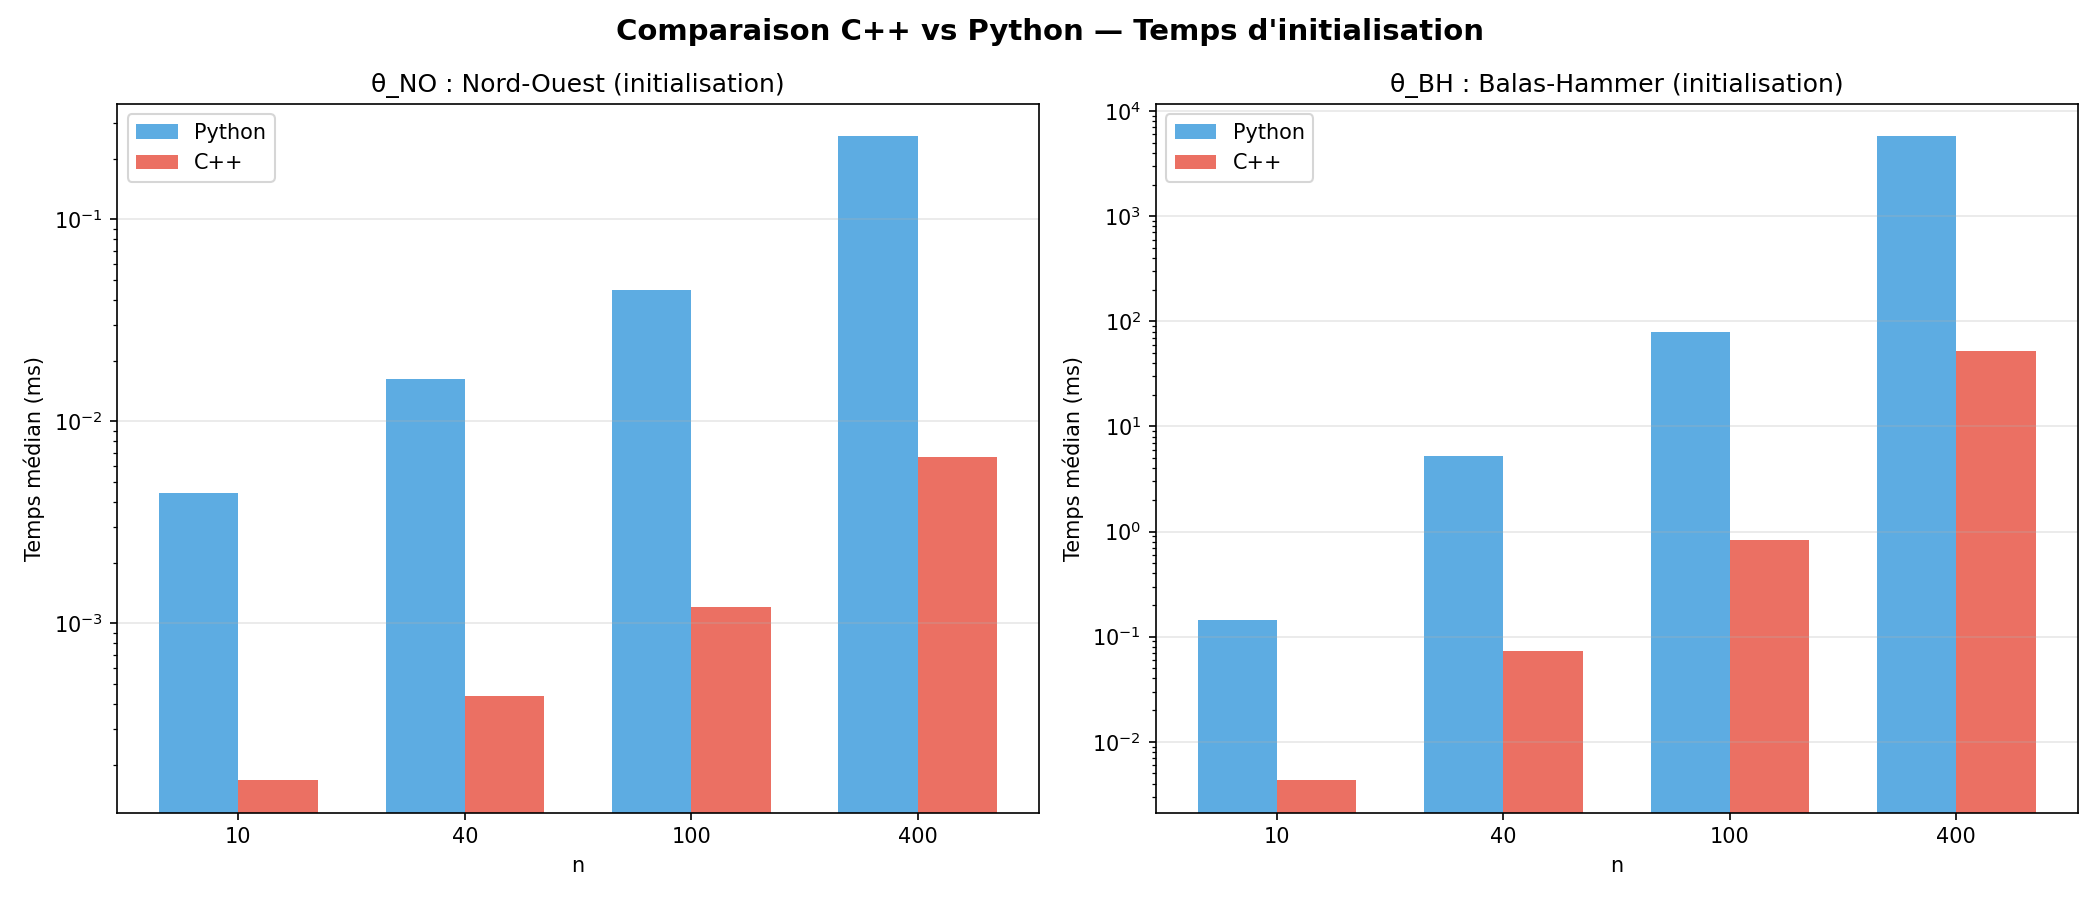
\includegraphics[width=\textwidth]{../results/figures/comparaison_initialisation.png}
\caption{Initialization time comparison -- C++ vs Python (log scale)}
\label{fig:init}
\end{figure}

\begin{table}[H]
\centering
\begin{tabular}{r|rrr|rrr}
\toprule
$n$ & Py $\theta_{\text{NO}}$ & C++ $\theta_{\text{NO}}$ & Speedup & Py $\theta_{\text{BH}}$ & C++ $\theta_{\text{BH}}$ & Speedup \\
\midrule
10  & 0.004 & 0.0002 & 26$\times$ & 0.145 & 0.004 & 34$\times$ \\
40  & 0.016 & 0.0004 & 37$\times$ & 5.23 & 0.072 & 72$\times$ \\
100 & 0.045 & 0.001 & 37$\times$ & 79.2 & 0.833 & 95$\times$ \\
400 & 0.258 & 0.007 & 39$\times$ & 5770 & 52.0 & 111$\times$ \\
\bottomrule
\end{tabular}
\caption{Initialization speedup -- C++ vs Python (median times in ms)}
\end{table}

\textbf{Key findings:}
\begin{itemize}
  \item For Nord-Ouest ($O(n)$), C++ is consistently $\sim$26--39$\times$ faster. The speedup is relatively stable because the algorithm is simple and memory-bound.
  \item For Balas-Hammer ($O(n^3)$), C++ speedup \emph{increases} with $n$: from 34$\times$ at $n=10$ to 111$\times$ at $n=400$. This is because the triple-nested loop structure benefits increasingly from compiler optimizations and cache locality.
\end{itemize}

\subsubsection{Stepping Stone Phase Comparison}

\begin{figure}[H]
\centering
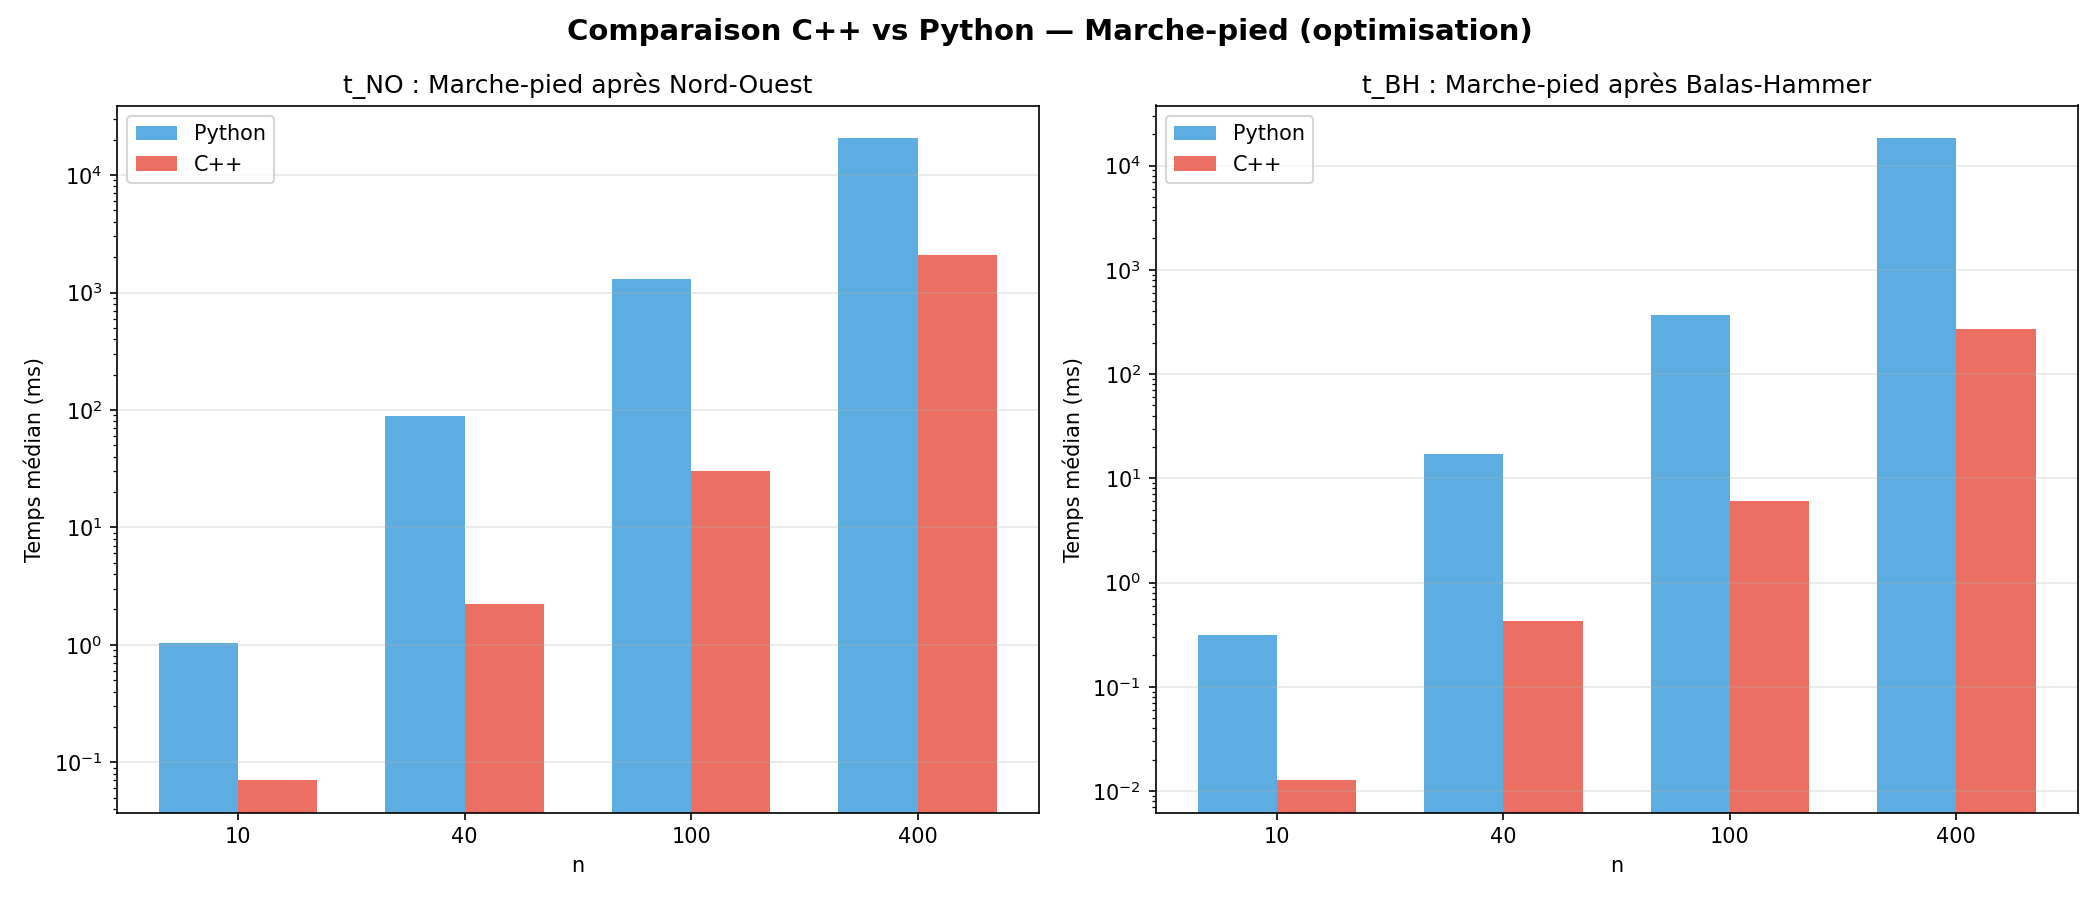
\includegraphics[width=\textwidth]{../results/figures/comparaison_marchepied.png}
\caption{Stepping Stone optimization time comparison -- C++ vs Python (log scale)}
\label{fig:stepping}
\end{figure}

\begin{table}[H]
\centering
\begin{tabular}{r|rrr|rrr}
\toprule
$n$ & Py $t_{\text{NO}}$ & C++ $t_{\text{NO}}$ & Speedup & Py $t_{\text{BH}}$ & C++ $t_{\text{BH}}$ & Speedup \\
\midrule
10  & 1.04 & 0.070 & 15$\times$ & 0.31 & 0.013 & 25$\times$ \\
40  & 89.0 & 2.23 & 40$\times$ & 17.2 & 0.43 & 40$\times$ \\
100 & 1299 & 30.3 & 43$\times$ & 371 & 6.04 & 62$\times$ \\
400 & 20842 & 2069 & 10$\times$ & 18522 & 269 & 69$\times$ \\
\bottomrule
\end{tabular}
\caption{Stepping Stone speedup -- C++ vs Python (median times in ms)}
\end{table}

\textbf{Key findings:}
\begin{itemize}
  \item Stepping Stone speedups range from 10$\times$ to 69$\times$, generally lower than initialization speedups. This is because the Stepping Stone method involves more complex control flow (graph traversal, cycle detection) that benefits less from simple loop optimizations.
  \item The anomalous drop in $t_{\text{NO}}$ speedup at $n=400$ (10$\times$) suggests that at this scale, both implementations become memory-bound, reducing the relative advantage of C++.
\end{itemize}

\subsubsection{Speedup Analysis}

\begin{figure}[H]
\centering
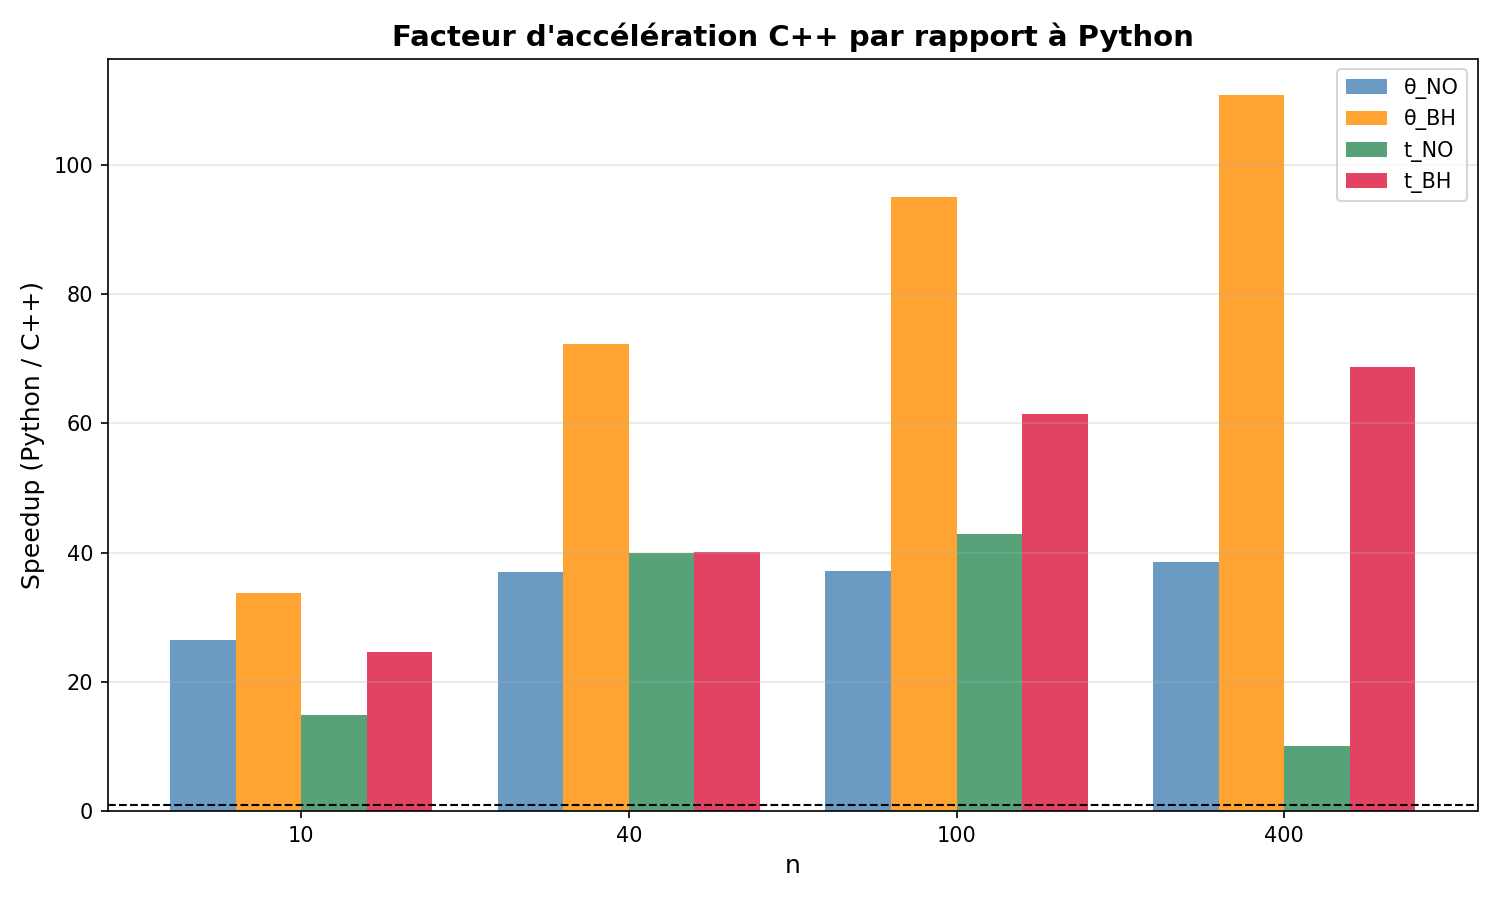
\includegraphics[width=0.85\textwidth]{../results/figures/comparaison_speedup.png}
\caption{C++ speedup factor over Python by algorithm phase and problem size}
\label{fig:speedup}
\end{figure}

The speedup chart reveals a clear pattern:
\begin{itemize}
  \item \textbf{$\theta_{\text{BH}}$ speedup grows with $n$}: The cubic algorithm amplifies the per-operation advantage of C++. Each additional nested loop level multiplies the benefit.
  \item \textbf{$\theta_{\text{NO}}$ speedup plateaus at $\sim$37--39$\times$}: The linear algorithm reaches a constant speedup determined by the language overhead ratio.
  \item \textbf{$t_{\text{BH}}$ speedup grows moderately}: The Stepping Stone benefits from C++ but less dramatically than pure initialization.
\end{itemize}

\subsubsection{Complexity Identification (Log-Log Analysis)}

\begin{figure}[H]
\centering
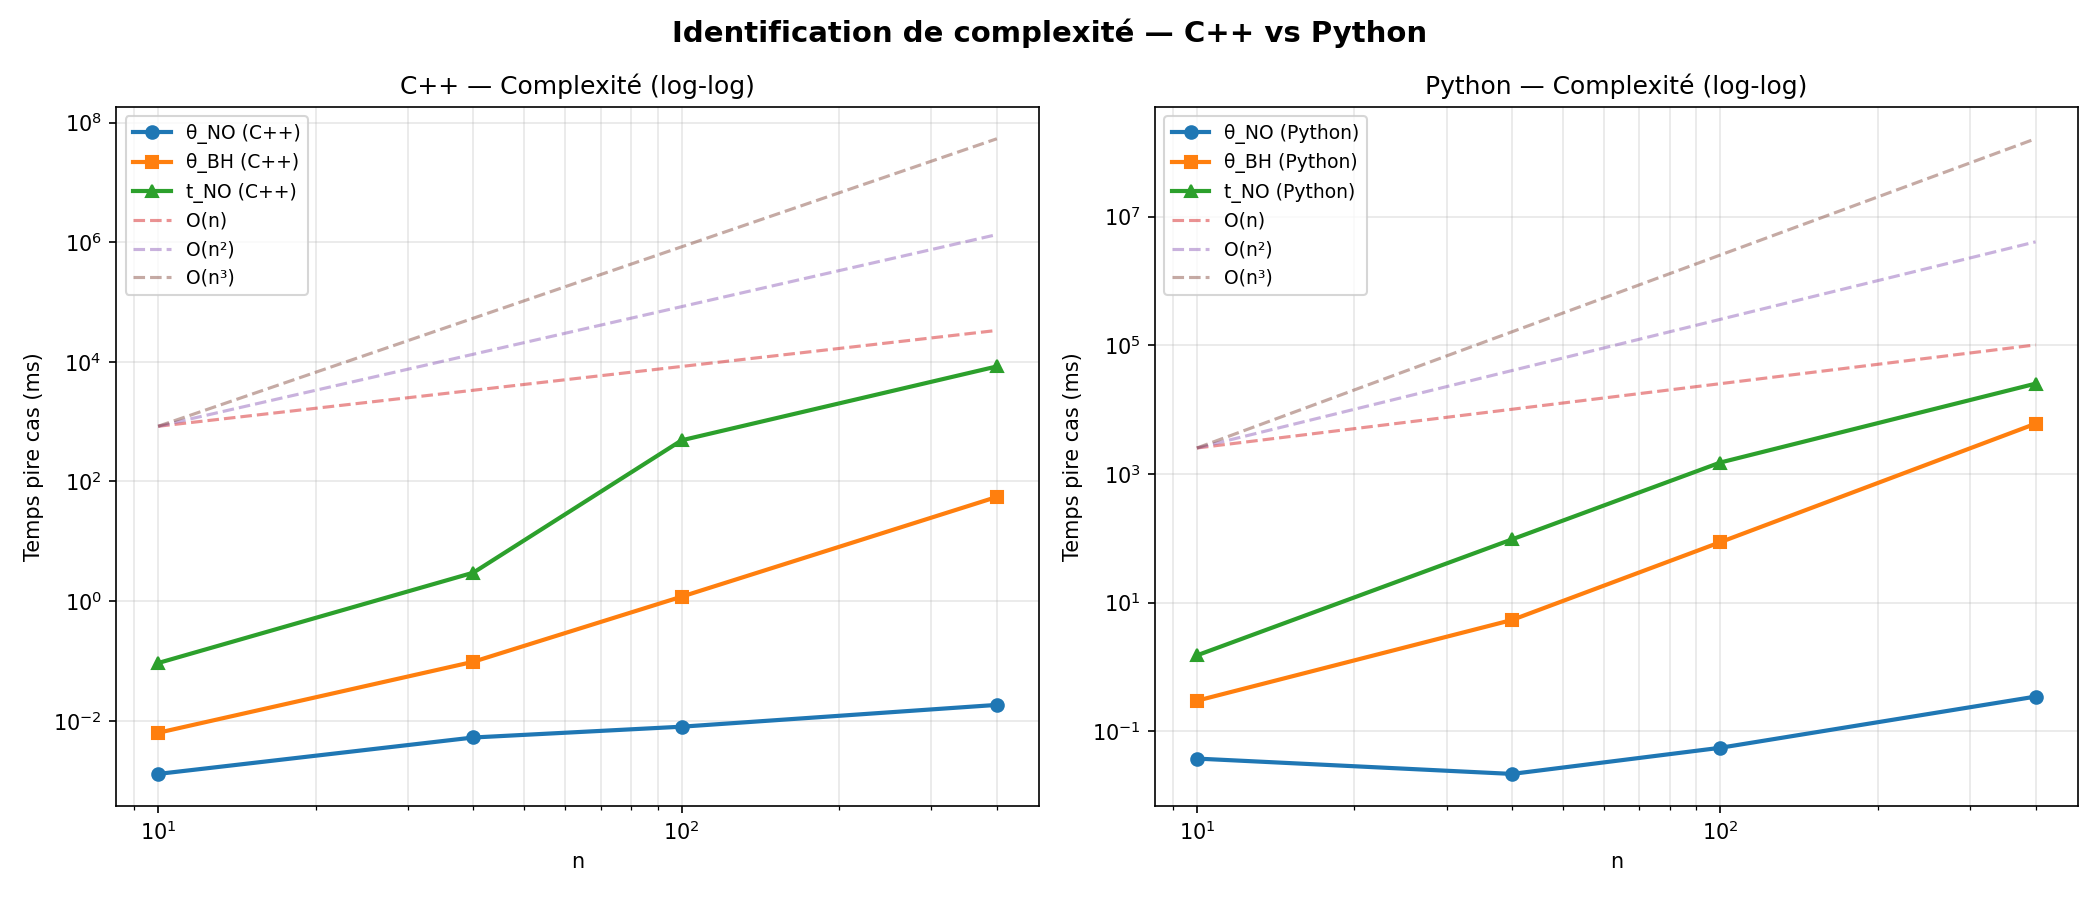
\includegraphics[width=\textwidth]{../results/figures/comparaison_loglog.png}
\caption{Log-log complexity analysis -- C++ (left) vs Python (right)}
\label{fig:loglog}
\end{figure}

The log-log plots confirm:
\begin{itemize}
  \item $\theta_{\text{NO}}$ follows $O(n)$ in both languages (slope $\approx 1$ on log-log).
  \item $\theta_{\text{BH}}$ follows $O(n^3)$ in both languages (slope $\approx 3$ on log-log).
  \item $t_{\text{NO}}$ and $t_{\text{BH}}$ fall between $O(n^2)$ and $O(n^3)$, consistent with the variable number of Stepping Stone iterations.
\end{itemize}

This confirms that \textbf{algorithmic complexity is language-independent}: both implementations exhibit the same asymptotic growth rates. The difference is purely in the constant factor.

\subsubsection{Total Time Comparison}

\begin{figure}[H]
\centering
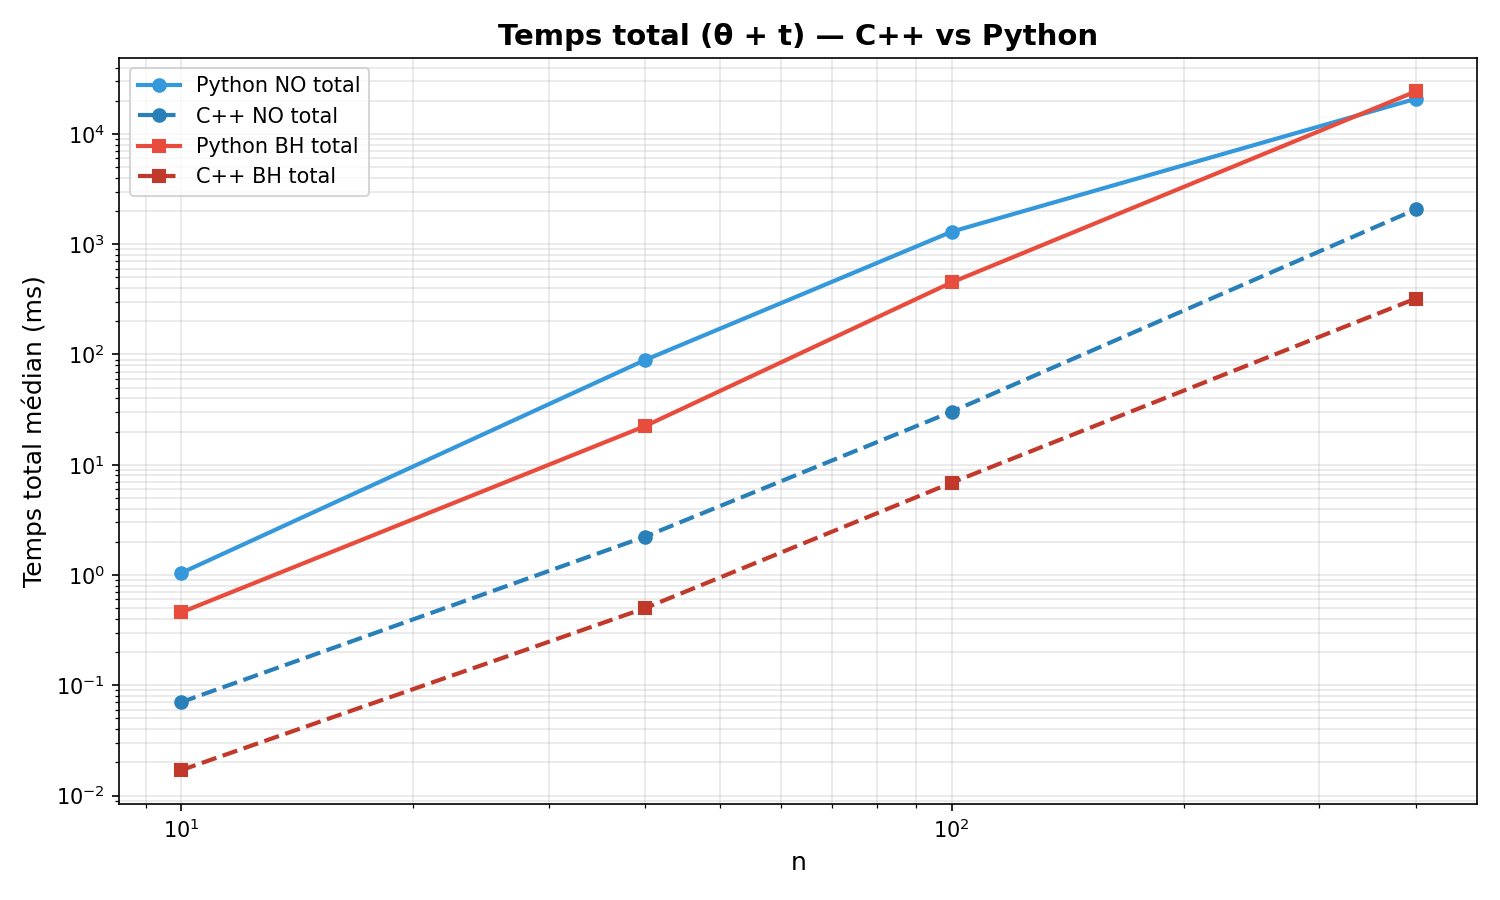
\includegraphics[width=0.85\textwidth]{../results/figures/comparaison_total.png}
\caption{Total time ($\theta + t$) -- C++ vs Python (log-log scale)}
\label{fig:total}
\end{figure}

The total time plot shows that:
\begin{itemize}
  \item C++ consistently outperforms Python across all sizes and methods.
  \item The BH path is slower than the NO path for large $n$ in both languages.
  \item The gap between Python and C++ widens with increasing $n$.
\end{itemize}

\subsection{Discussion}

\subsubsection{Why Does C++ Speedup Vary?}

The variable speedup factor (10$\times$ to 111$\times$) can be explained by several factors:

\begin{enumerate}
  \item \textbf{Interpreter overhead}: Python's bytecode interpretation adds a constant overhead per operation ($\sim$100\,ns). For simple operations (additions, comparisons), this dominates the actual computation time.
  \item \textbf{Dynamic typing}: Python's duck typing requires runtime type checks that C++ resolves at compile time.
  \item \textbf{Memory layout}: Python lists are arrays of pointers to heap-allocated objects. C++ \texttt{std::vector<int>} stores values contiguously, enabling CPU cache prefetching and SIMD vectorization.
  \item \textbf{Algorithm intensity}: The more operations per data element, the more the per-operation overhead compounds. This explains why BH (cubic) shows larger speedups than NO (linear).
\end{enumerate}

\subsubsection{Algorithmic vs.\ Language Optimization}

An important insight from this study:

\begin{quote}
\textit{Choosing a better algorithm (BH over NO for initialization) provides a better initial solution but at a higher cost. Choosing a faster language (C++ over Python) reduces execution time by a constant factor across all algorithms. These are orthogonal optimization axes.}
\end{quote}

For practical applications:
\begin{itemize}
  \item If $n$ is small ($\leq 100$), Python with BH initialization is sufficient.
  \item If $n$ is large ($\geq 1000$) and performance matters, C++ with NO initialization may be the best trade-off.
  \item For the best of both worlds, C++ with BH initialization provides optimal initial solutions at acceptable speed for all tested sizes.
\end{itemize}

% ══════════════════════════════════════════════════
% CONCLUSION
% ══════════════════════════════════════════════════
\newpage
\section{General Conclusion}

This study achieved its dual objective:

\textbf{1. Algorithmic comparison:} The Nord-Ouest algorithm is a lightweight $O(n)$ initialization method that produces suboptimal starting solutions, while Balas-Hammer is a more intelligent $O(n^3)$ method that produces significantly better initial solutions. The Stepping Stone optimization phase converges to the same optimal solution regardless of the starting point, but requires more iterations (and thus more time) from a poor starting point. The total solve time trade-off depends on problem size.

\textbf{2. Language comparison:} C++ outperforms Python by a factor of 10$\times$ to 111$\times$ across all tested configurations. The speedup is not constant -- it increases with algorithmic complexity and problem size, due to the compounding effect of per-operation overhead in interpreted languages. However, both languages exhibit the same asymptotic complexity, confirming that algorithmic analysis is implementation-independent.

\textbf{3. Practical recommendation:} For production-grade optimization solvers handling large-scale transportation problems, a compiled language is strongly recommended. For prototyping, analysis, and moderate-scale problems, Python remains the tool of choice due to its development speed and ecosystem.

\subsection{Limitations and Future Work}

\begin{itemize}
  \item The benchmark was limited to $n \leq 400$ for the full comparison due to Python's extreme slowness at larger sizes. The original Python-only complexity study tested up to $n = 10000$ but was not replicated in the cross-language benchmark.
  \item The C++ implementation does not use parallelism (OpenMP, SIMD intrinsics) beyond what the compiler auto-vectorizes. Manual parallelization could further improve performance.
  \item Alternative algorithms (Hungarian method, simplex network method) were not compared.
  \item The study uses randomly generated balanced problems; real-world unbalanced or sparse problems may exhibit different performance characteristics.
\end{itemize}

\vfill

\begin{center}
\rule{0.5\textwidth}{0.4pt}\\[0.5cm]
\textit{YAO Paul-Alex -- EFREI Paris -- Operations Research -- May 2026}
\end{center}

\end{document}
